\documentclass[12pt]{article}
\usepackage{preamble}

\pagestyle{fancy}
\fancyhead[LO,LE]{Дополнительные главы \\ высшей математики}
\fancyhead[RO,RE]{Лекции Далевской О. П.}

\fancyfoot[L]{\scriptsize исходники найдутся тут: \\ \url{https://github.com/pelmesh619/itmo_conspects} \Cat}

\renewcommand{\thesection}{}

\begin{document}

    \tableofcontents
    \clearpage

    % begin addchapters2_2025_02_07.tex





\section{1. Основные понятия}

\subsection{1.1. Комплексное число}

\Mem $\mathbb{C} = \{ (a, b) \ | \ a, b \in \Real\}$

Обозначение: $z = (a, b) = a + bi$, где $i = (0, -1) = \sqrt{-1}$

\underline{Основные операции}:

\begin{enumerate}
    \item $\mathrm{Re} z = a$ - вещественная часть, $\mathrm{Im} z = b$ - мнимая часть
    \item $z_1 + z_2 = (a_1, b_1) + (a_2, b_2) = (a_1 + a_2, b_1 + b_2) = (a_1 + a_2) + i(b_1 + b_2)$
    \item $z_1 \cdot z_2 = (a_1 + b_1 i) * (a_2 + b_2 i) = (a_1 a_2 - b_1 b_2) + i (a_1 b_2 + a_2 b_1)$
    \item $z^n = \rho^n (\cos n\varphi + i \sin n\varphi)$ - \textbf{формула Муавра}, где $\rho = |z|, \varphi = \arg z$
    \item $\sqrt[n]{z} = \sqrt[n]{\rho} \left(\cos \frac{\varphi + 2\pi k}{n} + i \sin \frac{\varphi + 2\pi k}{n}\right)$, где $\rho = |z|, \varphi = \arg z, k \in \mathbb{Z}$
    \item При $n = 2$ $\sqrt{z} = \sqrt{a + bi} = \pm (c + di)$, 
        где $c = \sqrt{\frac{a + \sqrt{a^2 + b^2}}{2}}, d = \mathrm{sign}(b) \sqrt{\frac{-a + \sqrt{a^2 + b^2}}{2}}$
\end{enumerate}

\begin{minipage}{\textwidth}
    % https://www.geogebra.org/calculator/xjg67fnv

    \begin{wrapfigure}{r}{0pt}
        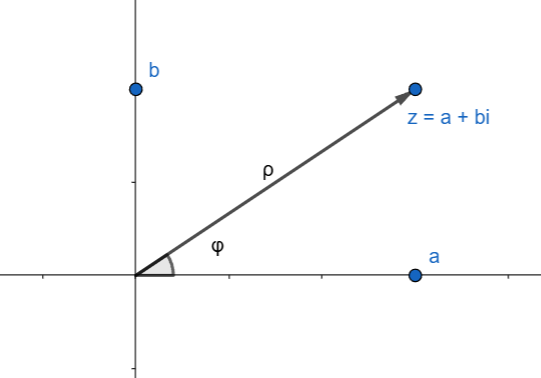
\includegraphics[width=7cm]{addchapters2/images/addchapters2_2025_02_07_6}
    \end{wrapfigure}

    Тригонометрическая форма:

    $z = a + bi = \rho (\cos \varphi + i \sin \varphi)$, где $\rho = |z| = \sqrt{a^2 + b^2}, \varphi = \arg z \in [0; 2\pi)$

    $\mathrm{Arg} z = \arg z + 2\pi k, k \in \mathbb{Z}$

    По формуле Эйлера $z = \rho (\cos \varphi + i \sin \varphi) = \rho e^{i \varphi}$
\end{minipage}

\subsection{1.2. Комплексная плоскость}

\Def Окрестность точки $z_0 \in \mathbb{C}$ определяется как $U_\delta (z_0) = \{z \in \mathbb{C} \ \Big| \ |z - z_0| < \delta\}$

Тогда $\overset{\circ}{U}_\delta (z_0) = U_\delta (z_0) \setminus \{ z_0 \}$ - выколотая окрестность

\Def Для данной множества точек $A$ точка $z_0$ считается

\begin{itemize}
    \item внутренней, если для любого $\delta$ $U_\delta (z_0) \subset A$
    \item граничной, если для любого $\delta$ $\exists z \in U_\delta (z_0) \Big| z \in A$ и $\exists z \in U_\delta (z_0) \Big| z \notin A$
\end{itemize}

\Def Открытое множество состоит только из внутренних точек

\Defs Закрытое множество содержит все свои граничные точки

\Defs Границой $\Gamma_D$ (иногда обозн. $\delta D$) для множества $D$ называют множество всех граничных точек $D$

\Defs Если любые две точки множества можно соединить ломаной линией конечной длины, то множество считается связным

\Defs Множество $D \subset \mathbb{C}$ называется областью, если $D$ - открытая и связная

\Defs Кривая $l \subset \mathbb{C}$ считается непрерывной, если $l = \{z \in \mathbb{C} \ | \ z = \varphi(t) + i \psi(t), t \in \Real\}$, где $\varphi(t), \psi(t)$ - непрерывные функции

\Notas Если $\varphi(t)$ и $\psi(t)$ дифференцируемы и их производные непрерывные, то кривая $l$ гладкая

\Defs Непрерывная замкнутая (то есть начальная и конечная точки совпадают) без самопересечений кривая называется контуром

\Notas Односвязную область можно стянуть в точку

% https://www.geogebra.org/calculator/nhbjhbag

\begin{multicols}{2}
    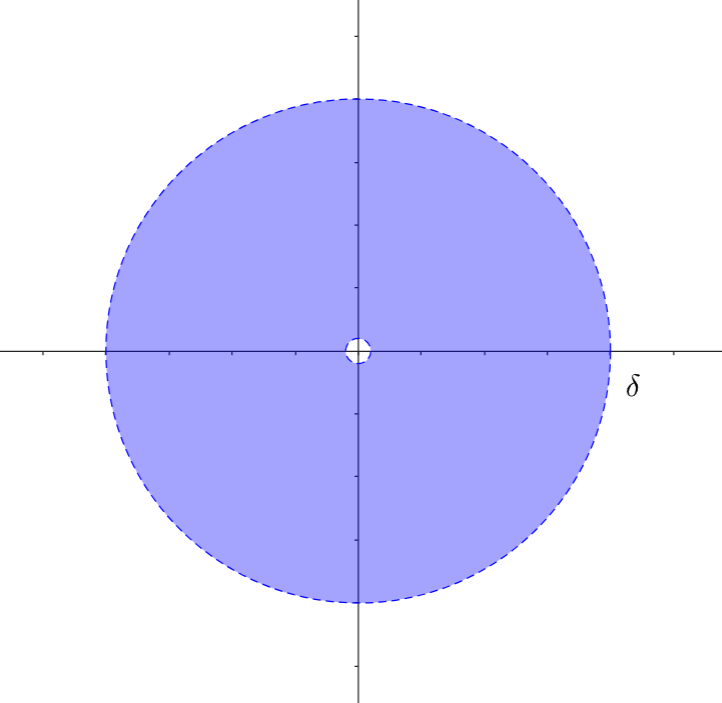
\includegraphics[width=0.4\textwidth]{addchapters2/images/addchapters2_2025_02_07_1}

    \ExNs{1} $D = \{z \in \mathbb{C} \ \Big| \ 0 < |z| < \delta\}$ - область связаная, но не односвязная, ее нельзя стянуть из-за дырки

    \mediumvspace

    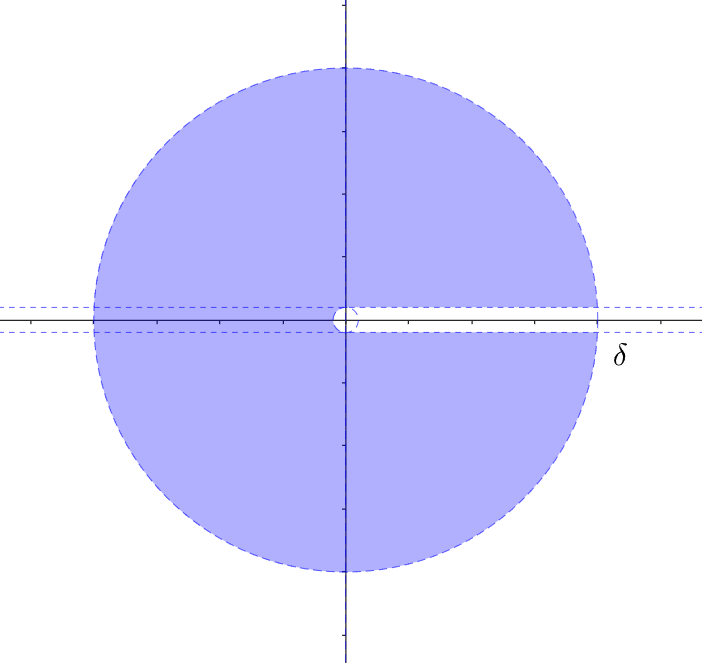
\includegraphics[width=0.4\textwidth]{addchapters2/images/addchapters2_2025_02_07_2}

    \ExN{2} $D = \{z \in \mathbb{C} \ \Big| \ 0 < |z| < \delta, \arg z \neq 0\}$ - область связная и односвязная
\end{multicols}

\begin{multicols}{2}
    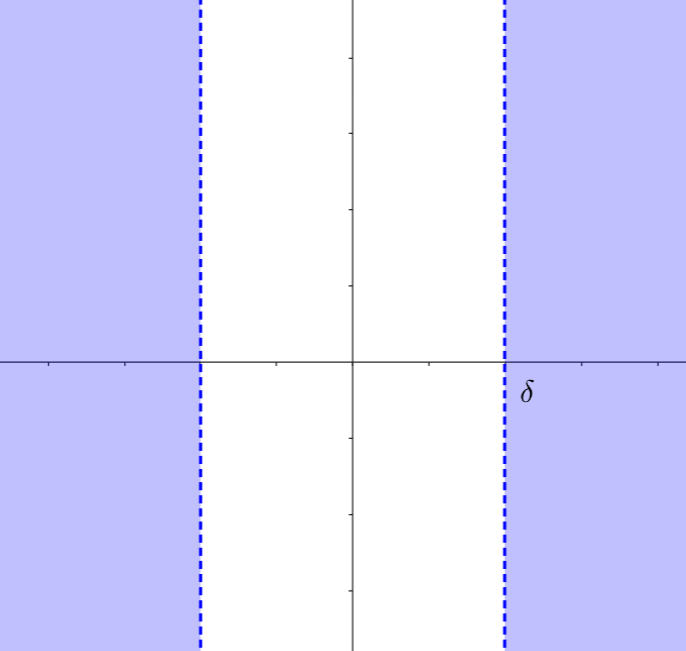
\includegraphics[width=0.4\textwidth]{addchapters2/images/addchapters2_2025_02_07_3}

    \ExN{3} $D = \{z \in \mathbb{C} \ \Big| \ |\mathrm{Re} z| < \delta\}$ - несвязная область

    \mediumvspace

    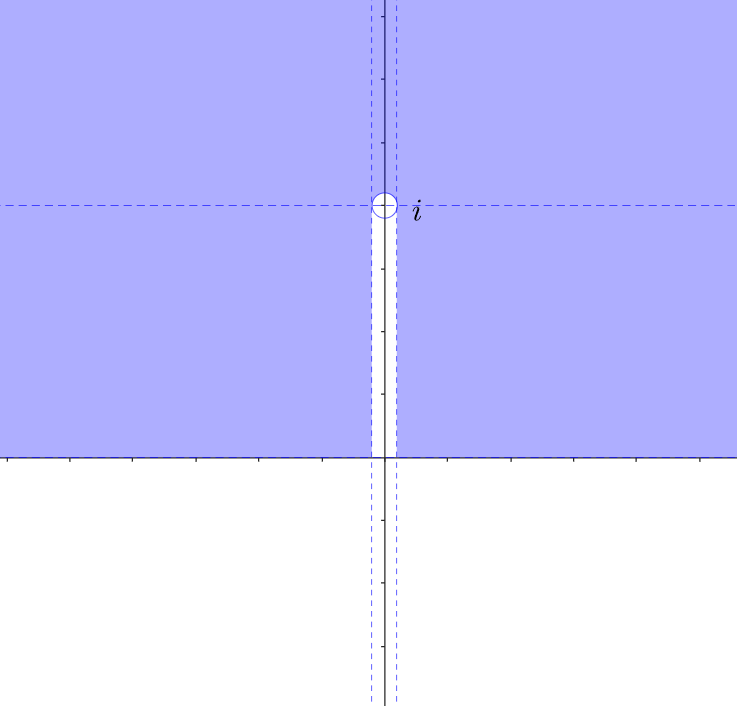
\includegraphics[width=0.4\textwidth]{addchapters2/images/addchapters2_2025_02_07_4}

    \ExN{4} $D = \{z \in \mathbb{C} \ \Big| \ \mathrm{Im} z \geq 0, z \notin [0, i]\}$ - здесь под $[0, i]$ подразумевается линейный отрезок на оси
\end{multicols}

\Nota Дальше все рассматриваемые $\Gamma_D$ будут состоять из кусочногладких и изолированных кривых

\subsection{1.3. Предел}

\Mem Последовательность $\{z_n\} = z_1, z_2, z_3, \dots, z_n, \dots$

\Def Пределом $\{z_n\}$ называют число $z$ такое, что

$\forall \varepsilon > 0 \ \exists \underset{n_0 = n_0(\varepsilon)}{n_0 = \Natural} \ \Big| \ \forall n > n_0 \ |z_n - z| < \varepsilon$

Обозначается $\lim_{n \to \infty} z_n = z$

\Nota $\{z_n\}$ можно представить как ${x_n + i y_n}$, то есть двумя $\Real$-последовательностями

\begin{MyTheorem}
    \Ths $\exists \lim_{n \to \infty} z_n = \underset{x, y \in \Real}{x + i y} \Longleftrightarrow $
    \begin{tabular}{l} $\exists \lim_{n \to \infty} x_n = \lim_{n \to \infty} \mathrm{Re} z_n = x$ \\ $\exists \lim_{n \to \infty} y_n = \lim_{n \to \infty} \mathrm{Im} z_n = y$ \end{tabular}
\end{MyTheorem}

\begin{MyProof}
    \fbox{$\Longleftarrow$} $\forall \varepsilon > 0 \ \exists \underset{n_0 = \max (n_{0x}, n_{0y})}{n_0 \in \Natural} \ \Big| \ \forall n > n_0 \begin{tabular}{l} |x_n - x| < \frac{\varepsilon}{2} \\ |y_n - y| < \frac{\varepsilon}{2} \end{tabular}$
    
    $|z_n - z| = |(x_n - x) + i(y_n - y)| \leq |x_n - x| + |y_n - y| < \frac{\varepsilon}{2} + \frac{\varepsilon}{2}$

    То есть $\forall \varepsilon > 0 \dots |z_n - z| < \varepsilon$

    \fbox{$\Longrightarrow$} $\forall \varepsilon > 0 \ |z_n - z| = |(x_n - x) + i(y_n - y)| < \varepsilon \Longrightarrow 
    \begin{cases}
        |x_n - x| \leq |(x_n - x) + i(y_n - y)| < \varepsilon \\
        |y_n - y| \leq |(x_n - x) + i(y_n - y)| < \varepsilon \\
    \end{cases} \Longrightarrow \exists \lim_{n \to \infty} x_n = x$ и $\exists \lim_{n \to \infty} y_n = y$

\end{MyProof}

\Nota Для комплексных чисел работают теоремы для пределов (сумма пределов, произведение пределов и т.д.), критерий Коши и другие

\Def $\lim_{n \to \infty} z_n = \infty \Longleftrightarrow \forall \varepsilon > 0 \ \exists \underset{n_0 = n_0(\varepsilon)}{n_0 \in \Natural} \ \Big| \ n > n_0 \ |z| > \varepsilon$

\Defs Точка $z$, определенная как предел, равный $\infty$, называется бесконечно удаленной. Но существует множество последовательностей, чьи пределы удаляются на бесконечность разными путями на плоскости

\Def Стереографическая проекция (сфера Римана)

% https://www.geogebra.org/calculator/kjesw2gx

\begin{center}
    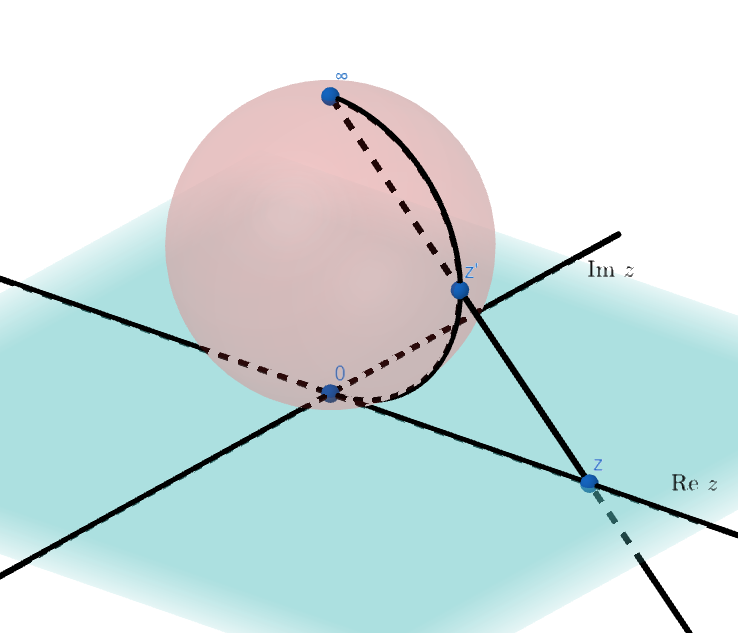
\includegraphics[width=0.55\textwidth]{addchapters2/images/addchapters2_2025_02_07_5}
\end{center}

Поместим сферу на комплексную плоскость и сделаем биекцию точек плоскости на точки сферы: проведем из верхней точки сферы лучи вниз на плоскость, и точка, где луч пересекает сфера,
будет считаться отображением для данной точки. Заметим, что в этом случае бесконечно удаленные точки будут отображаться в верхнюю точку сферы

\Def $\mathbb{C} \cup \{\infty\} = \overline{\mathbb{C}}$ - расширенная комплексная плоскость

Однако $z + \infty$ не определена, $\infty + \infty$ не определена. 
Но $\infty = \lim_{n \to \infty} \frac{1}{z_n}$ при $z_n \underset{n \to \infty}{\longrightarrow} 0$; $\infty = \infty \cdot \lim_{n \to \infty} z_n$ при $z_n \longrightarrow z$

Записью $[-\infty; +\infty]$ обозначается ось $\overline{\Real}$; 

\qquad\qquad $[-i\infty; +i\infty]$ - мнимая расширенная ось

Путь $x \pm i \infty$ при фикс. $x$ - вертикальная прямая; 

\qquad\qquad $iy \pm \infty$ - горизонтальная прямая; 

\qquad\qquad $e^{i\varphi} \cdot \infty$ - прямая, проходящая через начало координат



% end addchapters2_2025_02_07.tex

% begin addchapters2_2025_02_21.tex





\subsection{1.4. Комплексная функция}

\subsubsection{1$^\circ$ Определение}

\Mem $f : E \subset \Real \longrightarrow D \subset \Real \ \overset{def}{\Longleftrightarrow} \ $ отображение такое, 
что $\forall x \in E \ \exists! y \in D \ | \ y = f(x)$

\Def $f : D \subset \mathbb{C} \longrightarrow G \subset \mathbb{C} \ \overset{def}{\Longleftrightarrow} \ $ отображение такое, 
что $\forall z \in D \ \exists w \in G \ | \ f(z) = w$

\Defs Если $\forall z \in D \ \exists! w \in G$, то $f$ называется однозначной функцией

\Defs Если $\forall z_1, z_2 \in D (z_1 \neq z_2) \Longrightarrow f(z_1) \neq f(z_2)$, 
то $f$ называется однолистной функцией

\ExN{1} $w = \sqrt{z}$ - неоднозначная функция

$\letsymbol z = 1 = 1 (\cos 0 + i \sin 0)$

$\sqrt{z} = \sqrt{1} \left(\cos \frac{2\pi k}{2} + i \sin \frac{2\pi k}{2}\right)$

$w_1 = 1, \quad w_2 = -1$

\ExN{2} $w = z^2$ - неоднолистная функция

$z_1 = 1, z_2 = -1 \qquad\qquad w(z_1) = w(z_2) = 1$

\Nota Если $f(z)$ однозначна и однолистна, то $f(z)$ - взаимно однозначное соответствие (биекция). Тогда $\exists g(x) \ | \ g(f(x)) = x$

Комплексную функцию $f(z)$ можно представить как $u(x, y) + i v(x, y)$, где $x + iy = z$

\Ex $w = z^2 = (x + iy)^2 = x^2 + 2ixy - y^2 = (x^2 - y^2) + i \cdot 2xy$

$u(x, y) = (x^2 - y^2), \qquad\qquad v(x, y) = 2xy$

\subsubsection{2$^\circ$ Предел}

\Def $L \in \mathbb{C}, f : D \longrightarrow G, \quad L \overset{def}{=} \lim_{z \to z_0} f(z) \Longrightarrow
\forall \varepsilon > 0 \ \exists \underset{\delta = \delta(\varepsilon)}{\delta > 0} \ \Big| \ z \in D, z \in U^\circ_\delta(z_0) \ f(x) \in U_\varepsilon(L)$

В определении существование и значение $L$ не должно зависеть от пути, по которому $z$ приближается к точке сгущения $z_0$.
Может быть так, что для любого направления стремления предел есть, но в общем смысле не существует

% https://www.geogebra.org/calculator/hgk25mjs

\begin{wrapfigure}{R}{0pt}
    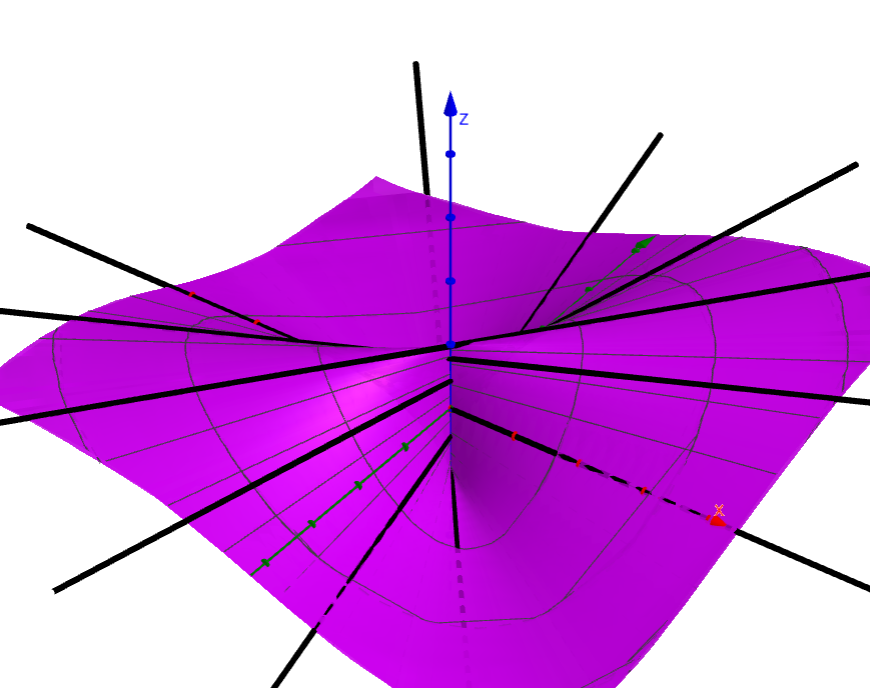
\includegraphics[width=7cm]{addchapters2/images/addchapters2_2025_02_21_2}
\end{wrapfigure}

\Ex $f(z) = \frac{1}{2i} \left(\frac{z}{\overline{z}} - \frac{\overline{z}}{z}\right) \qquad\qquad \letsymbol z = \rho e^{i\varphi}$

$f(z) = \frac{1}{2i} \left(\frac{\rho e^{i\varphi}}{\rho e^{-i\varphi}} - \frac{\rho e^{-i\varphi}}{\rho e^{i\varphi}}\right) =
\frac{1}{2i} \left(e^{2i\varphi} - e^{-2i\varphi}\right) = \frac{1}{2i} (\cos 2\varphi + i\sin 2\varphi - \cos 2\varphi + i\sin 2\varphi) = \sin 2\varphi$

Зафиксируем $\varphi = \varphi^* \in [0; 2\pi)$, тогда $\sin 2\varphi^* \in [-1; 1]$

$\lim_{z \to 0} f(z) = \lim_{\substack{\rho \to 0 \\ \varphi = \varphi^*}} f(z) = 
\lim_{\substack{\rho \to 0 \\ \varphi = \varphi^*}} \sin 2\varphi = \sin 2\varphi^* \in [-1; 1]$

Значения предела занимает отрезок $[-1; 1] \Longrightarrow \not\exists \lim_{z \to 0} f(z)$

На рисунке изображена $\sin 2\varphi$, на оси $Oz$ изображена $\mathrm{Re} w$. Черные линии - это возможные пути приближения $z$ к $0$

\Nota Путь следования предела аналогичен левостороннему и правостороннему пределами $\Real$-функций

\DefN{Непрерывность функций в точке $z_0$}

$f : D \longrightarrow G, z_0 \in D$, $f(z)$ называется непрерывной в $z_0$, если $\lim_{z \to z_0} f(z) = f(z_0)$

На языке приращений: $\Delta f = f(z_0 + \Delta z) - f(z_0) \underset{\Delta z \to 0}{\longrightarrow} 0$

$\Delta z = z - z_0 = \Delta x + i \Delta y \to 0 \Longrightarrow 
\begin{cases}\Delta x \to 0 \\ \Delta y \to 0\end{cases} \Longrightarrow 
\Delta \rho \to 0$

\subsubsection{3$^\circ$ Элементарные комплексные функции}

\ExN{1} Линейная $f(z) = az + b, \qquad\qquad a, b \in \mathbb{C} \quad a \neq 0$

Эта функция однозначная, однолистная $\Longrightarrow \exists f^{-1}(z) = g(z) = \frac{z - b}{a}$

\underline{Геометрический смысл}:

$a \in \mathbb{C}, z \in \mathbb{C}$

$az = |a| |z| (\cos (\varphi_a + \varphi_z) + i \sin (\varphi_a + \varphi_z))$ - поворот и растяжение 
($\varphi_a = \mathrm{arg} a$, $\varphi_z = \mathrm{arg} z$)

$az + b = (x_{az} + x_b) + i (y_{az} + y_b)$ - сдвиг

То есть линейная функция - композиция из поворота, растяжения и сдвига

\ExN{2} Степенная $w = z^n, \quad n \in \Natural$ - однозначная, может быть неоднолистной

Для $n \in \mathbb{Q}$ функция становится неоднозначной

\Exs $w = z^2 \qquad\qquad z = \rho e^{i\varphi}, w = \rho^2 e^{2i\varphi}$

Пусть $z_1 \neq z_2$ и $w(z_1) = w(z_2)$, тогда $\mathrm{arg} z_1 = \mathrm{arg} z_2 \pm \pi$ 

$w(z_1) = \rho^2 e^{2i\mathrm{arg} z_1} = \rho^2 e^{2i (\mathrm{arg} z_1 + 2\pi k)}$

$w(z_2) = \rho^2 e^{2i\mathrm{arg} z_2} = \rho^2 e^{2i (\mathrm{arg} z_1 + \pi)} = \rho^2 e^{i (2\mathrm{arg} z_1 + 2\pi)} = w(z_1)$

Область однолистности $z^2$ - множество точек, для которых $\mathrm{arg} z \in [0; \pi)$

Точку $w = 0$ называют точкой разветвления

% https://www.geogebra.org/calculator/phuam9sh

\begin{wrapfigure}{r}{0pt}
    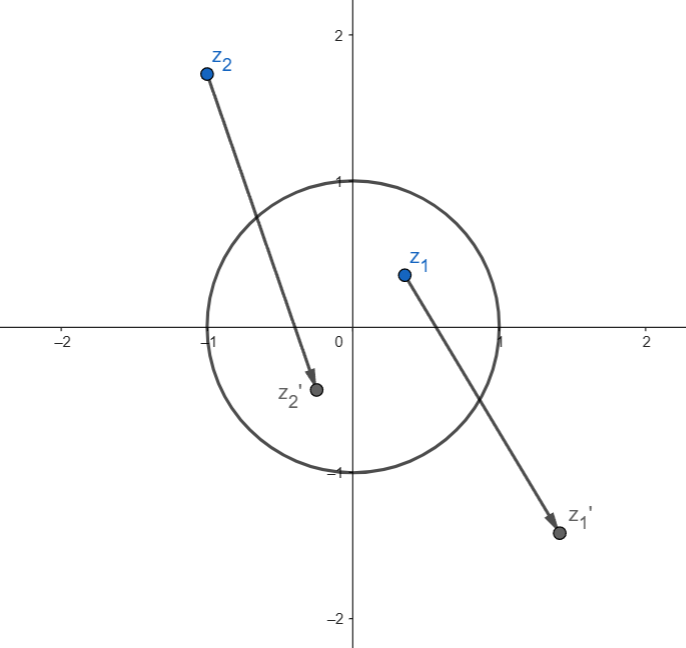
\includegraphics[width=7cm]{addchapters2/images/addchapters2_2025_02_21_1}
\end{wrapfigure}

\Exs $w = z^{-1} = \frac{1}{z} \qquad\qquad w(0) = \infty, w(\infty) = 0$

$z \in \mathbb{C} \setminus \{0\}$ - функция обратима

$w = re^{i\psi} = \frac{1}{\rho e^{i\phi}} = \frac{1}{\rho} e^{-i\varphi} \Longrightarrow |w| = \frac{1}{|z|}, \mathrm{arg} w = -\mathrm{arg} z$

Преобразование $|w| = \frac{1}{|z|}$ называется инверсией, а $\mathrm{arg} w = -\mathrm{arg} z$ дает симметрию относительно $\mathrm{Re} z$

\ExN{3} Рациональная $f(z) = \frac{P_n(z)}{Q_m(z)}, \qquad\qquad n, m \in \Natural$

\ExN{4} Показательная $w = e^z = e^x \cdot e^{iy} = e^x (\cos y + i \sin y)$

\underline{Свойства}: 

\begin{enumerate}
    \item $e^{z_1 + z_2} = e^{z_1} \cdot e^{z_2}$
    \item $\left(e^{z_1}\right)^{z_2} = e^{z_1 z_2}$
    \item $e^{z + 2\pi i} = e^{z} \cdot e^{2\pi i} = e^z$ - показательная функция периодична с периодом $2\pi i$
\end{enumerate}

\ExN{5} Логарифмическая $w = \mathrm{Ln} z$

Если $e^w = e^{u + vi} = e^u (\cos v + i \sin v) = z = |z| e^{i\mathrm{arg} z}$, то $u = \ln |z|$, $v = \mathrm{arg} z + 2\pi k$

Тогда \fbox{$\mathrm{Ln} z = \ln |z| (\cos (\mathrm{arg} z + 2\pi k) + i \sin (\mathrm{arg} z + 2\pi k))$}

$\ln z = \mathrm{Ln} z$ при $k = 0$ - т. н. главное значение




% end addchapters2_2025_02_21.tex



\end{document}

